\appendix{Представление графического материала}

Графический материал, выполненный на отдельных листах,
изображен на рисунках А.1--А.\arabic{числоПлакатов}.
\setcounter{числоПлакатов}{0}

\renewcommand{\thefigure}{А.\arabic{figure}} % шаблон номера для плакатов

\begin{landscape}

\begin{плакат}
    
\includegraphics[width=0.82\linewidth]{плакат1.eps}
    \заголовок{Сведения о ВКРБ}
    \label{pl1:image}      
\end{плакат}

\begin{плакат}
	
\includegraphics[width=0.82\linewidth]{плакат2.eps}
	\заголовок{Цель и задачи разработки}
	\label{pl2:image}      
\end{плакат}

\begin{плакат}
	
\includegraphics[width=0.82\linewidth]{плакат3.eps}
	\заголовок{Диограмма прецедентов}
	\label{pl3:image}      
\end{плакат}

\begin{плакат}
	
\includegraphics[width=0.82\linewidth]{плакат4.eps}
	\заголовок{Диограмма компонентов}
	\label{pl4:image}      
\end{плакат}

\begin{плакат}
    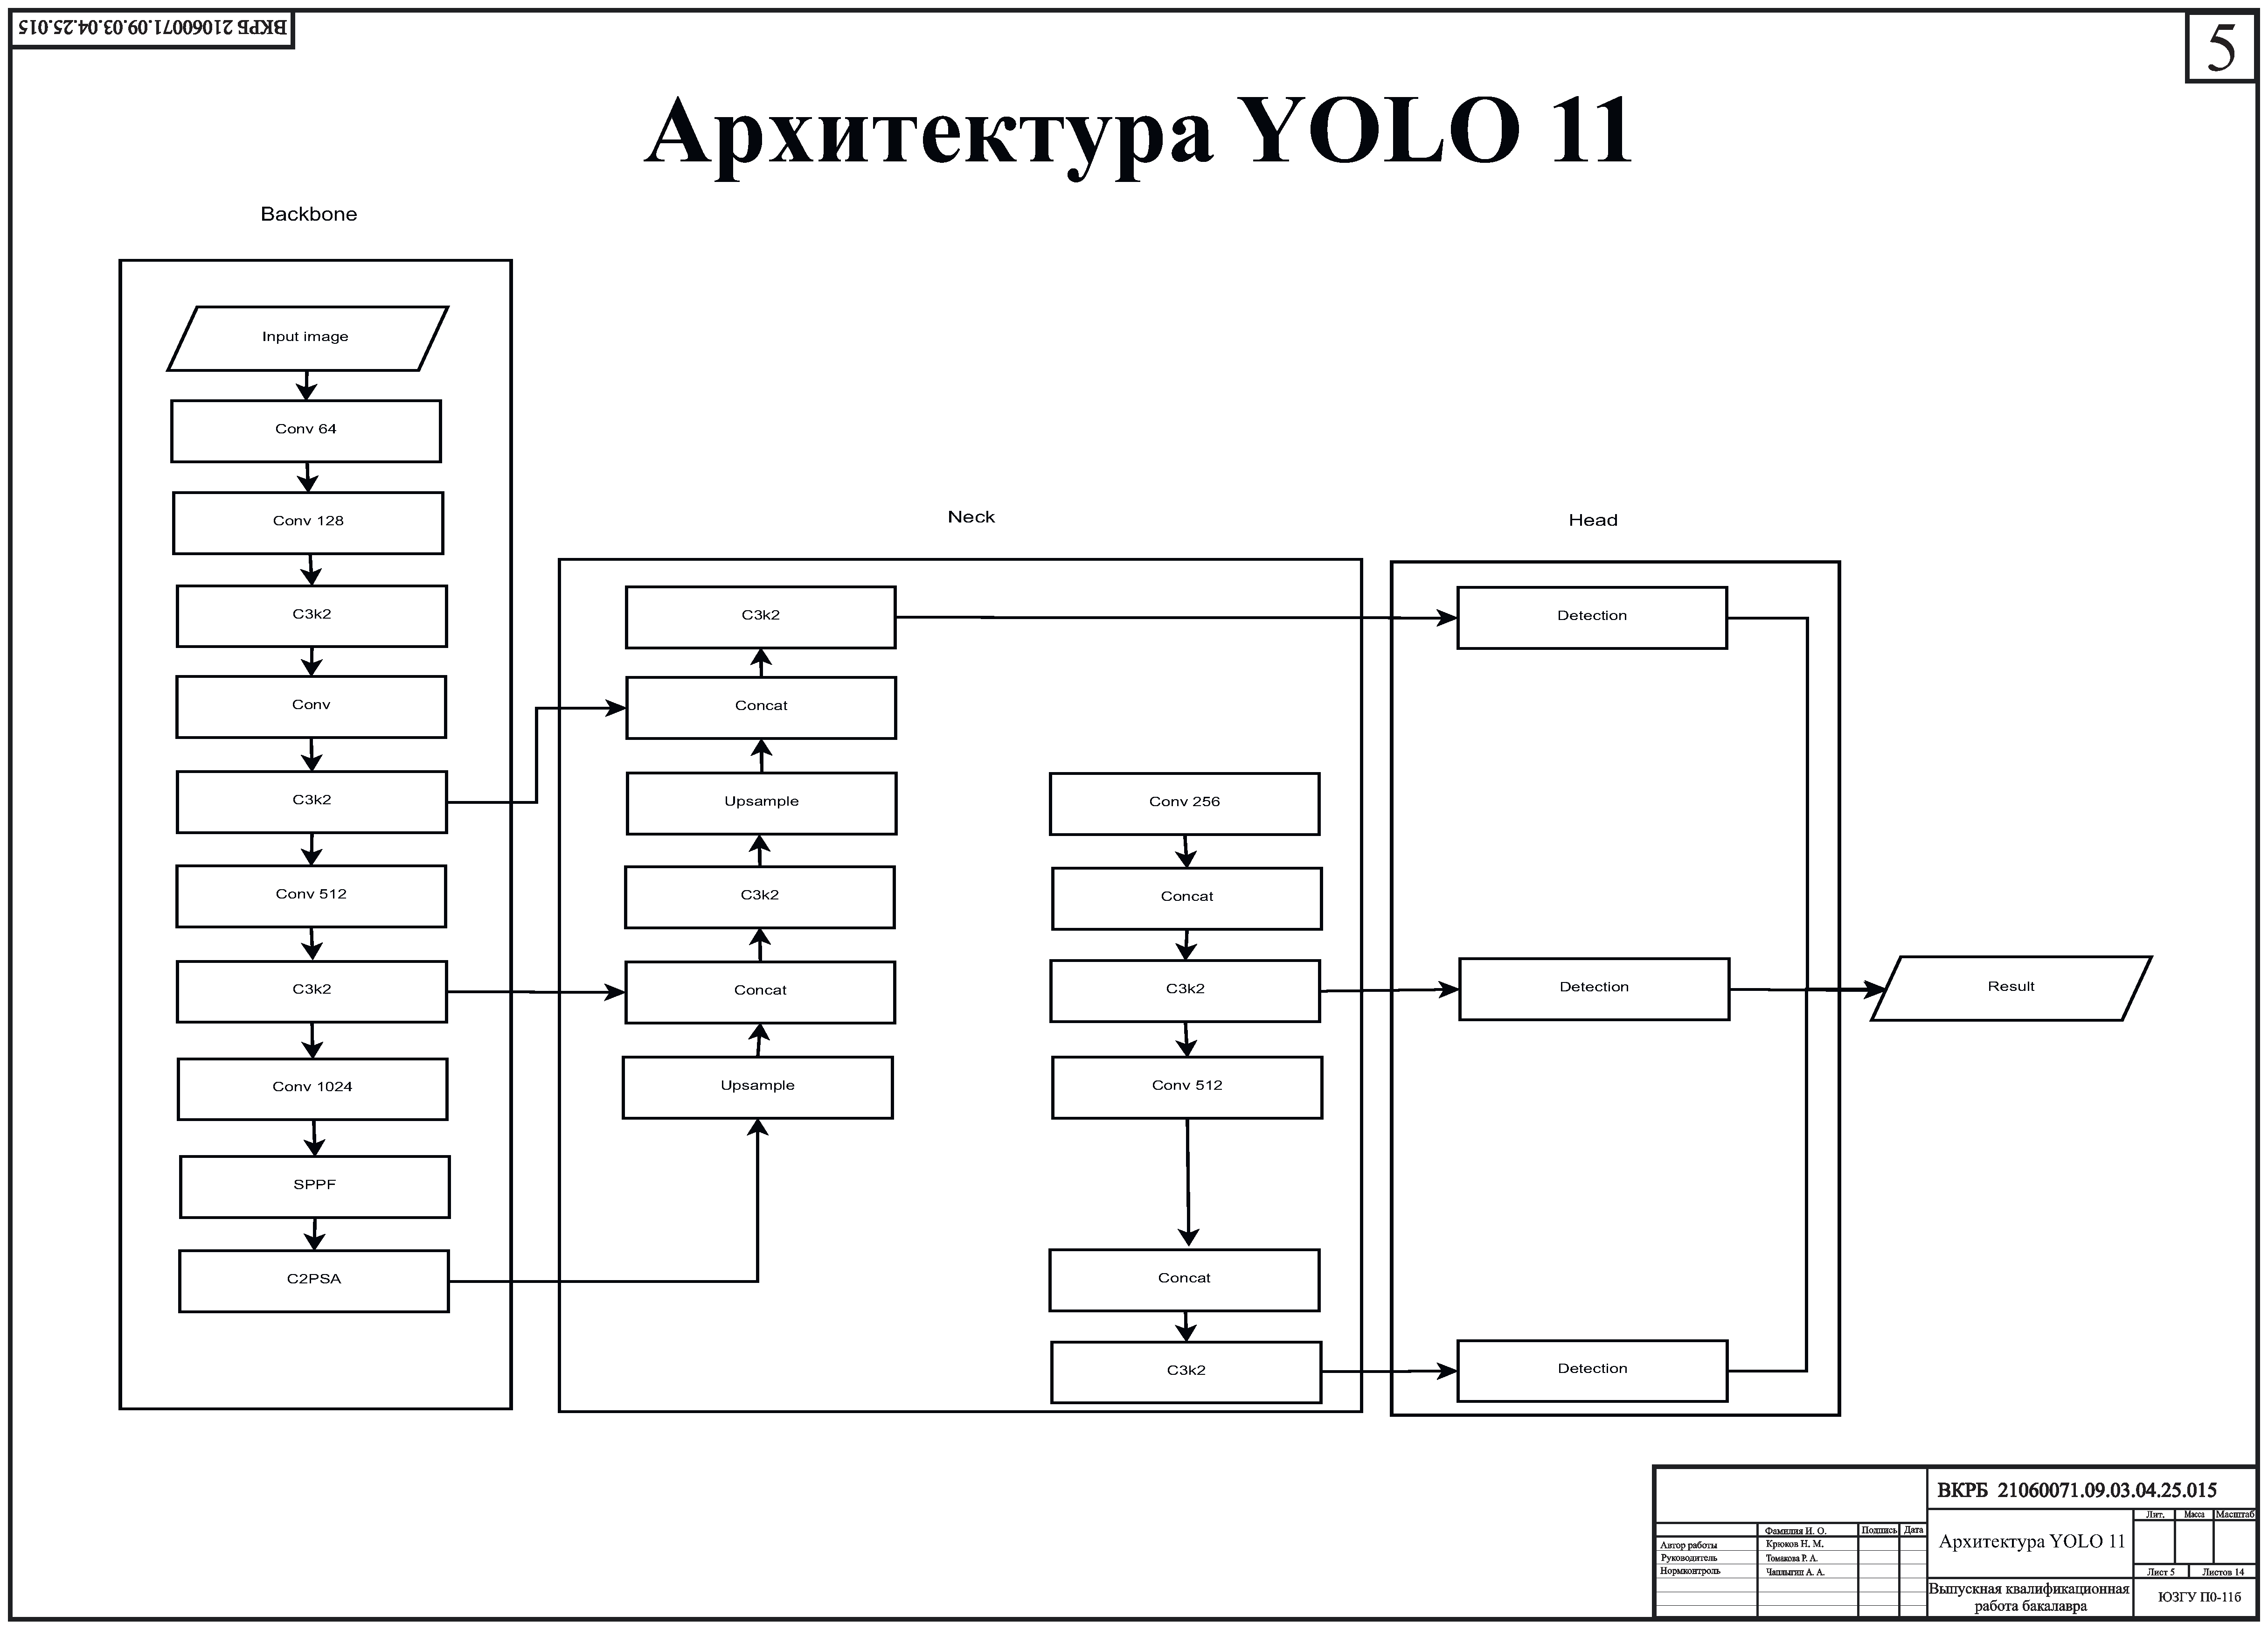
\includegraphics[width=0.82\linewidth]{плакат5.eps}
    \заголовок{Архитектура YOLO 11}
    \label{pl5:image}      
\end{плакат}

\begin{плакат}
	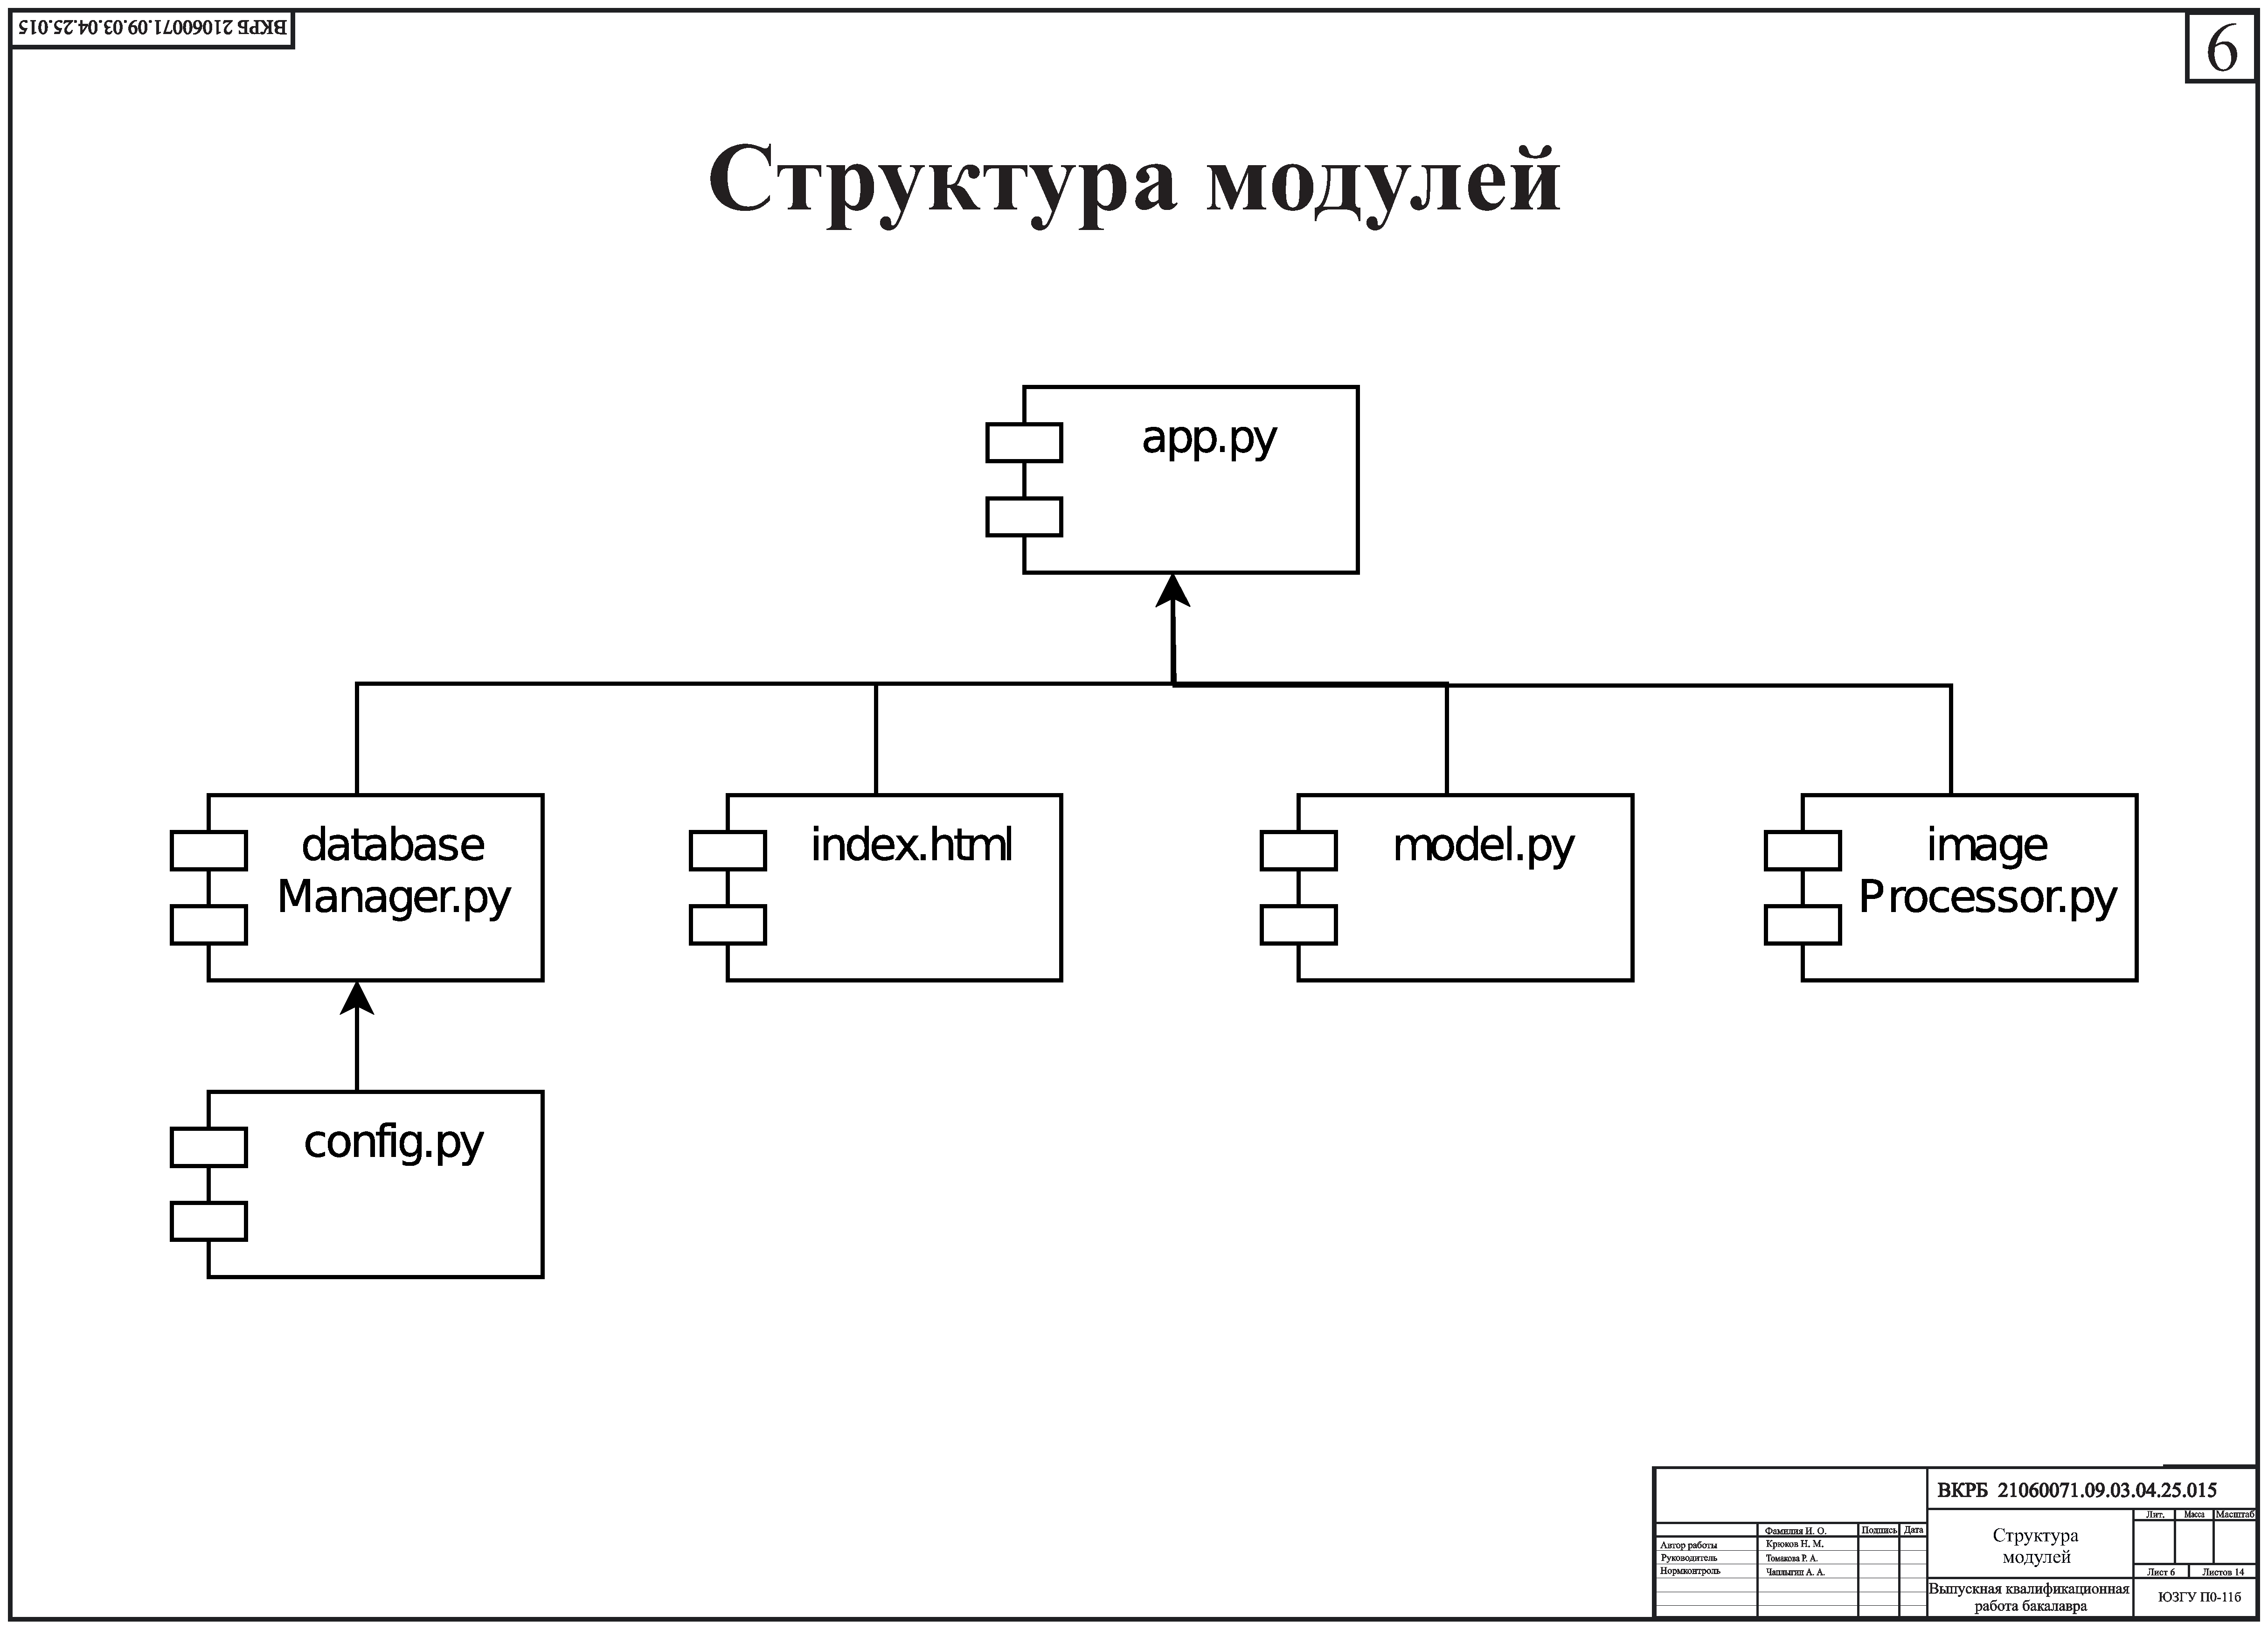
\includegraphics[width=0.82\linewidth]{плакат6.eps}
	\заголовок{Структура модулей}
	\label{pl:6image}      
\end{плакат}

\begin{плакат}
	
\includegraphics[width=0.82\linewidth]{плакат7.eps}
	\заголовок{Динамика метрик обучения}
	\label{pl:7image}      
\end{плакат}

\begin{плакат}
	
\includegraphics[width=0.82\linewidth]{плакат8.eps}
	\заголовок{Кривые F1-меры в зависимости от порога уверенности}
	\label{pl:8image}      
\end{плакат}

\begin{плакат}
	
\includegraphics[width=0.82\linewidth]{плакат9.eps}
	\заголовок{Кривые точности и полноты}
	\label{pl:9image}      
\end{плакат}

\begin{плакат}
	
\includegraphics[width=0.82\linewidth]{плакат10.eps}
	\заголовок{Нормализованная матрица ошибок}
	\label{pl:10image}      
\end{плакат}

\begin{плакат}
	
\includegraphics[width=0.82\linewidth]{плакат11.eps}
	\заголовок{Результат анализа фотографии}
	\label{pl:11image}      
\end{плакат}

\begin{плакат}
	
\includegraphics[width=0.82\linewidth]{плакат12.eps}
	\заголовок{Описание болезни}
	\label{pl:12image}      
\end{плакат}

\begin{плакат}
	
\includegraphics[width=0.82\linewidth]{плакат13.eps}
	\заголовок{Методы лечения и профилактики}
	\label{pl:13image}      
\end{плакат}

\begin{плакат}
	
\includegraphics[width=0.82\linewidth]{плакат14.eps}
	\заголовок{Заключение}
	\label{pl:14image}      
\end{плакат}

\end{landscape}
